\documentclass[sunil1,ChapterTOCs]{sunil}
\usepackage[utf8]{inputenc}
\usepackage{amssymb}
\usepackage{amsmath}
\usepackage{graphicx}
\usepackage{subfigure}
%\usepackage{epsfig}
\usepackage{makeidx}
\usepackage{listings}
\usepackage{caption}
\usepackage{courier}
\usepackage{color}
\usepackage[sectionbib]{bibunits}
\usepackage{multicol}
\usepackage{alltt}


\frenchspacing
\tolerance=5000

\include{Chapters/chapter1/preamble}

\makeatletter


\makeatother

\newtheorem{proposition}{Proposition}
\newtheorem{proof}{Proof}




 \lstset{
         basicstyle=\footnotesize\ttfamily, % Standardschrift
         %numbers=left,               % Ort der Zeilennummern
         numberstyle=\tiny,          % Stil der Zeilennummern
         %stepnumber=2,               % Abstand zwischen den Zeilennummern
         numbersep=5pt,              % Abstand der Nummern zum Text
         tabsize=2,                  % Groesse von Tabs
         extendedchars=true,         %
         breaklines=true,            % Zeilen werden Umgebrochen
         keywordstyle=\color{red},
    		frame=b,         
 %        keywordstyle=[1]\textbf,    % Stil der Keywords
 %        keywordstyle=[2]\textbf,    %
 %        keywordstyle=[3]\textbf,    %
 %        keywordstyle=[4]\textbf,   \sqrt{\sqrt{}} %
         stringstyle=\color{white}\ttfamily, % Farbe der String
         showspaces=false,           % Leerzeichen anzeigen ?
         showtabs=false,             % Tabs anzeigen ?
         xleftmargin=17pt,
         framexleftmargin=17pt,
         framexrightmargin=5pt,
         framexbottommargin=4pt,
         %backgroundcolor=\color{lightgray},
         showstringspaces=false      % Leerzeichen in Strings anzeigen ?        
 }
 \lstloadlanguages{% Check Dokumentation for further languages ...
         %[Visual]Basic
         %Pascal
         C
         %C++
         %XML
         %HTML
         %Java
 }
  %\DeclareCaptionFont{blue}{\color{blue}} 

  %\captionsetup[lstlisting]{singlelinecheck=false, labelfont={blue}, textfont={blue}}
\DeclareCaptionFont{white}{\color{white}}
\DeclareCaptionFormat{listing}{\colorbox[cmyk]{0.43, 0.35, 0.35,0.01}{\parbox{\textwidth}{\hspace{15pt}#1#2#3}}}
\captionsetup[lstlisting]{format=listing,labelfont=white,textfont=white, singlelinecheck=false, margin=0pt, font={bf,footnotesize}}



\makeindex

\begin{document}


%%bibliography style to adopt
\bibliographyunit[\chapter]
\defaultbibliographystyle{plain}



\title{Designing Scientific Applications on GPUs }

\author{Raphaël Couturier}

\maketitle

\frontmatter
\chapter*{Foreward}
I am delighted to introduce the first book on Multimedia Data Mining.  When I came to know about this book project undertaken by two of the most active young researchers in the field, I was pleased that this book is coming in early stage of a field that will need it more than most fields do.  In most emerging research fields, a book can play a significant role in bringing some maturity to the field.  Research fields advance through research papers.  In research papers, however, only a limited perspective could be provided about the field, its application potential, and the techniques required and already developed in the field.  A book gives such a chance.  I liked the idea that there will be a book that will try to unify the field by bringing in disparate topics already available in several papers that are not easy to find and understand.  I was supportive of this book project even before I had seen any material on it.  The project was a brilliant and a bold idea by two active researchers.  Now that I have it on my screen, it appears to be even a better idea.  

Multimedia started gaining recognition in 1990s as a field.  Processing, storage, communication, and capture and display technologies had advanced enough that researchers and technologists started building approaches to combine information in multiple types of signals such as audio, images, video, and  text.  Multimedia computing and communication techniques recognize correlated information in multiple sources as well as insufficiency of information in any individual source.    By properly selecting sources to provide complementary information, such systems aspire, much like human perception system, to create a holistic picture of a situation using only partial information from separate sources.

Data mining is a direct outgrowth of progress in data storage and processing speeds.  When it became possible to store large volume of data and run different statistical computations to explore all possible and even unlikely correlations among data, the field of data mining was born.  Data mining allowed people to hypothesize relationships among data entities and explore support for those.  This field has been put to applications in many diverse domains and keeps getting more applications.  In fact many new fields are direct outgrowth of data mining and it is likely to become a powerful computational tool.\vadjust{\vfill\pagebreak}

\thispagestyle{empty}


\include{frontmatter/preface}

\listoffigures
\listoftables
\tableofcontents

\mainmatter

\include{Chapters/symbollist}

\setcounter{page}{1}
\part{This is a Part}
%\chapterauthor{Raphaël Couturier}{Femto-ST Institute, University of Franche-Comte}


\chapter{Presentation of the GPU architecture and of the Cuda environment}
\label{chapter1}

\section{Introduction}\label{ch1:intro}

This chapter introduces the Graphics  Processing Unit (GPU) architecture and all
the concepts needed to understand how GPUs  work and can be used to speed up the
execution of some algorithms. First of all this chapter gives a brief history of
the development  of Graphics  card until they  have been  used in order  to make
general   purpose   computation.    Then   the   architecture  of   a   GPU   is
illustrated.  There  are  many  fundamental  differences between  a  GPU  and  a
tradition  processor. In  order  to benefit  from the  power  of a  GPU, a  Cuda
programmer needs to use threads. They have some particularities which enable the
Cuda model to be efficient and scalable when some constraints are addressed.



\section{Brief history of Video Card}

Video  cards or Graphics  cards have  been introduced  in personal  computers to
produce  high quality graphics  faster than  classical Central  Processing Units
(CPU) and  to alleviate CPU from this  task. In general, display  tasks are very
repetitive and very specific.  Hence,  some manufacturers have produced more and
more sophisticated video cards, providing 2D accelerations then 3D accelerations,
then some  light transforms. Video cards  own their own memory  to perform their
computation.  For at least two decades, every personal computer has had a video
card which is simple for  desktop computers or which provides many accelerations
for game and/or  graphic oriented computers.  In the  latter case, graphic cards
may be more expensive than a CPU.

Since  2000, video  cards have  allowed  users to  apply arithmetic  operations
simultaneously on a sequence of  pixels, also later called stream processing. In
this case, the information of the pixels (color, location and other information) are
combined in order  to produce a pixel  color that can be displayed  on a screen.
Simultaneous  computations are  provided  by shaders  which calculate  rendering
effects on  graphics hardware with a  high degree of  flexibility. These shaders
handles the stream data with pipelines.


Some researchers  tried to  apply those operations  on other  data, representing
something different  from pixels,  and consequently this  resulted in  the first
uses of video cards for  performing general purpose computation. The programming
model  was not  easy  to use  at  all and  was very  dependent  of the  hardware
constraints.   More precisely  it consisted  in using  either DirectX  of OpenGL
functions  providing  an  interface  to  some classical  operations  for  videos
operations  (memory  transfers,  texture  manipulation,  ...).   Floating  point
operations were  most of the  time unimaginable.  Obviously when  something went
wrong, programmers had no way (and neither the tools) to detect it.

\section{GPGPU}

In order  to benefit from the computing  power of more recent  video cards, Cuda
was first proposed in 2007 by  NVidia. It unifies the programming model for some
of  their most performant  video cards.   Cuda~\cite{ch1:cuda} has  quickly been
considered by  the scientific community as  a great advance  for general purpose
graphics processing unit (GPGPU)  computing.  Of course other programming models
have been  proposed. The  other well-known alternative  is OpenCL which  aims at
proposing an alternative to Cuda  and which is multi-platform and portable. This
is a  great advantage since  it is even  possible to execute OpenCL  programs on
traditional CPUs.  The main drawback is that it is less tight with the hardware
and  consequently sometimes  provides  less efficient  programs. Moreover,  Cuda
benefits from  more mature compilation and optimization  procedures.  Other less
known environments  have been proposed, but  most of them have  been stopped, for
example  we can  cite: FireStream  by ATI  which is  not maintained  anymore and
replaced by  OpenCL, BrookGPU by  Standford University~\cite{ch1:Buck:2004:BGS}.
Another environment based  on pragma (insertion of pragma  directives inside the
code to  help the compiler to generate  efficient code) is call  OpenACC.  For a
comparison with OpenCL, interested readers may refer to~\cite{ch1:CMR:12}.



\section{Architecture of current GPUs}

The architecture  \index{architecture of  a GPU} of  current GPUs  is constantly
evolving.  Nevertheless  some trends remain constant  throughout this evolution.
Processing units composing a GPU are  far more simple than a traditional CPU but
it is much easier to integrate many computing units inside a GPU card than to do
so with many cores inside a CPU. This is due to the fact that the cores of a GPU are
simpler than the cores of a CPU.  In  2012, the most powerful GPUs own more than 500
cores       and       the       most       powerful      CPUs       have       8
cores. Figure~\ref{ch1:fig:comparison_cpu_gpu} shows  the number of cores inside
a  CPU  and  inside a  GPU.   In  fact,  in  a  current NVidia  GPU,  there  are
multiprocessors which have 32 cores (for example on Fermi cards). The core clock
of CPU is  generally around 3GHz and  the one of GPU is  about 1.5GHz.  Although
the core clock of GPU cores is slower, the amount of cores inside a GPU provides
more computational power.  This measure is commonly represented by the number of
floating point operation  per seconds. Nowadays the most powerful  GPUs provide more
than   1TFlops,  i.e.    $10^{12}$   floating  point   operations  per   second.
Nevertheless  GPUs are very  efficient to  perform some  operations but  not all
kinds of operations. They are very efficient to execute repetitive work in which
only  the data  change. It  is important  to keep  in mind  that multiprocessors
inside a GPU have 32 cores. Later we will see that these 32 cores need to do the
same work to get maximum performance.

\begin{figure}[b!]
\centerline{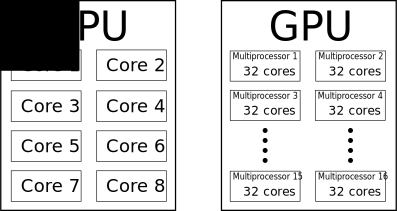
\includegraphics[]{Chapters/chapter1/figures/nb_cores_CPU_GPU.pdf}}
\caption{Comparison of number of cores in a CPU and in a GPU.}
%[Comparison of number of cores in a CPU and in a GPU]
\label{ch1:fig:comparison_cpu_gpu}
\end{figure}

On the most powerful  GPU cards, called Fermi, multiprocessors  are called streaming
multiprocessors  (SM). Each  SM contains  32  cores and  is able  to perform  32
floating points or integer operations on  32 bits numbers per clock or 16 floating
points  on  64 bits number  per  clock. SMs  have  their  own registers,  execution
pipelines and caches.  On Fermi architecture,  there are 64Kb shared memory + L1
cache  and 32,536 32bits  registers per  SM. More  precisely the  programmer can
decide what amount  of shared memory and  L1 cache SM can use.  The constraint is
that the sum of both amounts should be less or equal to 64Kb.

Threads are used to  benefit from the important number of cores  of a GPU. Those
threads    are   different    from    traditional   threads    for   CPU.     In
chapter~\ref{chapter2},  some  examples of  GPU  programming  will explicit  the
details of  the GPU  threads. However,  threads are gathered  into blocks  of 32
threads, called ``warps''. Those warps  are important when designing an algorithm
for GPU.


Another big  difference between CPU and GPU  is the latency of  memory.  In CPU,
everything is optimized  to obtain a low latency  architecture. This is possible
through  the  use  of  cache  memories. Moreover,  nowadays  CPUs  perform  many
performance optimizations  such as speculative execution  which roughly speaking
consists in executing  a small part of  code in advance even if  later this work
reveals itself  to be  useless. On the  contrary, GPUs  do not have  low latency
memory.   In comparison GPUs  have small  cache memories.  Nevertheless the
architecture of GPUs is optimized  for throughput computation and it takes into
account the memory latency.



\begin{figure}[b!]
\centerline{\includegraphics[scale=0.7]{Chapters/chapter1/figures/low_latency_vs_high_throughput.pdf}}
\caption{Comparison of low latency of CPU and high throughput of GPU.}
\label{ch1:fig:latency_throughput}
\end{figure}

Figure~\ref{ch1:fig:latency_throughput}  illustrates   the  main  difference  of
memory latency between a CPU and a  GPU. In a CPU, tasks ``ti'' are executed one
by one with a short memory latency to get the data to process. After some tasks,
there is  a context switch  that allows the  CPU to run  concurrent applications
and/or multi-threaded  applications. Memory latencies  are longer in a  GPU, the
the  principle  to   obtain  a  high  throughput  is  to   have  many  tasks  to
compute. Later we  will see that those tasks are called  threads with Cuda. With
this  principle, as soon  as a  task is  finished the  next one  is ready  to be
executed  while the  wait for  data for  the previous  task is  overlapped by
computation of other tasks.



\section{Kinds of parallelism}

Many  kinds  of parallelism  are  amiable according  to  the  type of  hardware.
Roughly  speaking, there  are three  classes of  parallelism: instruction-level
parallelism, data parallelism and task parallelism.

Instruction-level parallelism consists in re-ordering some instructions in order
to execute  some of them in parallel  without changing the result  of the code.
In  modern CPUs, instruction  pipelines allow  processor to  execute instructions
faster.   With   a  pipeline  a  processor  can   execute  multiple  instructions
simultaneously due  to the fact that  the output of a  task is the  input of the
next one.

Data parallelism consists  in executing the same program  with different data on
different computing  units.  Of course,  no dependency should exist  between the
data. For example, it is easy  to parallelize loops without dependency using the
data parallelism paradigm. This paradigm  is linked with the Single Instructions
Multiple Data (SIMD)  architecture. This is the kind  of parallelism provided by
GPUs.

Task parallelism is the common parallelism  achieved out on clusters and grids and
high performance  architectures where different tasks are  executed by different
computing units.

\section{Cuda Multithreading}

The data parallelism  of Cuda is more precisely based  on the Single Instruction
Multiple Thread (SIMT) model. This is due to the fact that a programmer accesses
to  the cores  by the  intermediate of  threads. In  the Cuda  model,  all cores
execute the  same set of  instructions but with  different data. This  model has
similarities with the vector programming  model proposed for vector machines through
the  1970s into  the  90s, notably  the  various Cray  platforms.   On the  Cuda
architecture, the  performance is  led by the  use of  a huge number  of threads
(from thousands up to  to millions). The particularity of the  model is that there
is no  context switching as in  CPUs and each  thread has its own  registers. In
practice,  threads  are executed  by  SM  and are  gathered  into  groups of  32
threads.  Those  groups  are  called  ``warps''. Each  SM  alternatively  executes
``active warps''  and warps becoming temporarily  inactive due to  waiting of data
(as shown in Figure~\ref{ch1:fig:latency_throughput}).

The key to scalability in the Cuda model is the use of a huge number of threads.
In practice, threads are not only gathered  in warps but also in thread blocks. A
thread block is executed  by only one SM and it cannot  migrate. The typical size of
a thread block is a number power of two (for example: 64, 128, 256 or 512).



In this  case, without changing anything inside  a Cuda code, it  is possible to
run your  code with  a small Cuda  device or  the most performing Tesla  Cuda cards.
Blocks are  executed in any order depending  on the number of  SMs available. So
the  programmer  must  conceive  its  code  having this  issue  in  mind.   This
independence between thread blocks provides the scalability of Cuda codes.

\begin{figure}[b!]
\centerline{\includegraphics[scale=0.65]{Chapters/chapter1/figures/scalability.pdf}}
\caption{Scalability of GPU.}
\label{ch1:fig:scalability}
\end{figure}


A kernel is a function which  contains a block of instructions that are executed
by the  threads of a GPU.   When the problem considered  is a two  dimensional or three
dimensional  problem,  it is  possible  to group  thread  blocks  into a grid.   In
practice, the number of  thread blocks and the size of thread  blocks is given as
parameters  to  each  kernel.   Figure~\ref{ch1:fig:scalability}  illustrates  an
example of a kernel composed of 8 thread blocks. Then this kernel is executed on
a small device containing only 2 SMs.  So in  this case, blocks are executed 2
by 2 in any order.  If the kernel is executed on a larger Cuda device containing
4 SMs, blocks are executed 4 by 4 simultaneously.  The execution times should be
approximately twice faster in the latter  case. Of course, that depends on other
parameters that will be described later.

Thread blocks provide a way to cooperation  in the sense that threads of the same
block   cooperatively    load   and   store   blocks   of    memory   they   all
use. Synchronizations of threads in the same block are possible (but not between
threads of different  blocks). Threads of the same block  can also share results
in order  to compute a  single result. In chapter~\ref{chapter2},  some examples
will explicit that.


\section{Memory hierarchy}

The memory hierarchy of  GPUs\index{memory~hierarchy} is different from the CPUs
one.  In practice,  there are registers\index{memory~hierarchy!registers}, local
memory\index{memory~hierarchy!local~memory},                               shared
memory\index{memory~hierarchy!shared~memory},                               cache
memory\index{memory~hierarchy!cache~memory}              and              global
memory\index{memory~hierarchy!global~memory}.


As  previously  mentioned each  thread  can access  its  own  registers.  It  is
important to keep in mind that the  number of registers per block is limited. On
recent cards,  this number is  limited to 64Kb  per SM.  Access to  registers is
very fast, so it is a good idea to use them whenever possible.

Likewise each thread can access local  memory which, in practice, is much slower
than registers.  Local memory is automatically used by the compiler when all the
registers are  occupied. So the  best idea is  to optimize the use  of registers
even if this implies to reduce the number of threads per block.

\begin{figure}[hbtp!]
\centerline{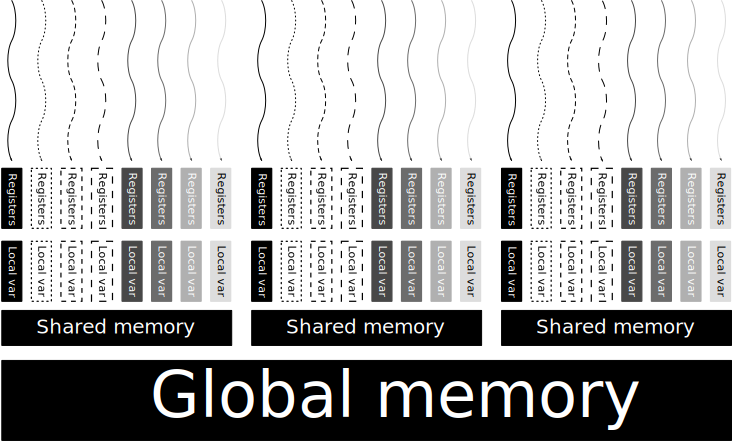
\includegraphics[scale=0.60]{Chapters/chapter1/figures/memory_hierarchy.pdf}}
\caption{Memory hierarchy of a GPU.}
\label{ch1:fig:memory_hierarchy}
\end{figure}



Shared memory allows  cooperation between threads of the  same block.  This kind
of memory is fast because it requires to be manipulated manually and its size is
limited.  It is accessible during the execution of a kernel. So the principle is
to fill the shared  memory at the start of the kernel  with global data that are
used very  frequently, then threads can  access it for  their computation.  They
can obviously change  the content of this shared  memory either with computation
or load of  other data and they can  store its content in the  global memory. So
shared memory can  be seen as a cache memory  manageable manually. This requires
obviously an effort from the programmer.

On  recent cards,  the programmer  may decide  what amount  of cache  memory and
shared memory is attributed to a kernel. The cache memory is a L1 cache which is
directly  managed by  the GPU.  Sometimes,  this cache  provides very  efficient
result and sometimes the use of shared memory is a better solution.




Figure~\ref{ch1:fig:memory_hierarchy}  illustrates  the  memory hierarchy  of  a
GPU. Threads are represented on the top  of the figure. They can access to their
own registers  and their local memory. Threads  of the same block  can access to
the shared memory of this block. The cache memory is not represented here but it
is local  to a thread. Then  each block can access  to the global  memory of the
GPU.

 \section{Conclusion}

In this chapter,  a brief presentation of the video card,  which has later been
used to perform computation, has been  given. The architecture of a GPU has been
illustrated focusing on the particularity of GPUs in term of parallelism, memory
latency and  threads. In order to design  an efficient algorithm for  GPU, it is
essential to have all these parameters in mind.


\putbib[Chapters/chapter1/biblio]


%\chapterauthor{Raphaël Couturier}{Femto-ST Institute, University of Franche-Comte}

\chapter{Introduction to Cuda}
\label{chapter2}

\section{Introduction}
\label{ch2:intro}

In this chapter  we give some simple examples of Cuda  programming.  The goal is
not to provide an exhaustive presentation of all the functionalities of Cuda but
rather to give some basic elements. Of  course, readers that do not know Cuda are
invited  to read  other  books that  are  specialized on  Cuda programming  (for
example: \cite{ch2:Sanders:2010:CEI}).


\section{First example}
\label{ch2:1ex}

This first example is  intented to show how to build a  very simple program with
Cuda.  Its goal  is to perform the sum  of two arrays and put the  result into a
third array.  A Cuda program consists in  a C code which calls Cuda kernels that
are executed on a GPU. The listing of this code is in Listing~\ref{ch2:lst:ex1}.


As GPUs have  their own memory, the first step consists  in allocating memory on
the GPU.  A call to  \texttt{cudaMalloc}\index{Cuda~functions!cudaMalloc} allows
to allocate memory on the GPU. The first parameter of this function is a pointer
on a memory on the device (i.e. the GPU). In this example, \texttt{d\_} is added
on each variable allocated  on the GPU, meaning this variable is  on the GPU. The
second parameter represents the size of the allocated variables, this size is expressed in
bits.

In this example, we  want to compare the execution time of  the additions of two
arrays in  CPU and  GPU. So  for both these  operations, a  timer is  created to
measure the  time. Cuda proposes to  manipulate timers quite  easily.  The first
step is to create the timer\index{Cuda~functions!timer}, then to start it and at
the end to stop it. For each of these operations a dedicated function is used.

In  order to  compute  the same  sum  with a  GPU, the  first  step consists  in
transferring the data from the CPU (considered as the host with Cuda) to the GPU
(considered as the  device with Cuda).  A call  to \texttt{cudaMemcpy} allows to
copy the content of an array allocated in the host to the device when the fourth
parameter                                 is                                 set
to  \texttt{cudaMemcpyHostToDevice}\index{Cuda~functions!cudaMemcpy}.  The first
parameter of the function is the  destination array, the second is the
source  array and  the third  is the  number of  elements to  copy  (expressed in
bytes).

Now the  GPU contains the  data needed to  perform the addition.   In sequential
programming, such  addition is  achieved out  with a loop  on all  the elements.
With a GPU,  it is possible to perform  the addition of all the  elements of the
two  arrays in  parallel (if  the number  of blocks  and threads  per  blocks is
sufficient).   In Listing\ref{ch2:lst:ex1}  at the  beginning, a  simple kernel,
called \texttt{addition} is defined to  compute in parallel the summation of the
two     arrays.      With     Cuda,     a     kernel     starts     with     the
keyword   \texttt{\_\_global\_\_}   \index{Cuda~keywords!\_\_shared\_\_}   which
indicates that this kernel can be called from the C code.  The first instruction
in this kernel is used to compute the variable \texttt{tid} which represents the
thread index.   This thread index\index{thread  index} is computed  according to
the           values            of           the           block           index
(called  \texttt{blockIdx} \index{Cuda~keywords!blockIdx}  in Cuda)  and  of the
thread   index   (called   \texttt{blockIdx}\index{Cuda~keywords!threadIdx}   in
Cuda). Blocks of threads and thread  indexes can be decomposed into 1 dimension,
2 dimensions or  3 dimensions.  According to the  dimension of manipulated data,
the appropriate dimension  can be useful. In our example,  only one dimension is
used.   Then using notation  \texttt{.x} we  can access  to the  first dimension
(\texttt{.y}  and \texttt{.z}  respectively allow to access  to the  second and
third dimension).   The variable \texttt{blockDim}\index{Cuda~keywords!blockDim}
gives the size of each block.



\lstinputlisting[label=ch2:lst:ex1,caption=A simple example]{Chapters/chapter2/ex1.cu}

\section{Second example: using CUBLAS}
\label{ch2:2ex}

The Basic Linear Algebra Subprograms  (BLAS) allows programmers to use efficient
routines  that are  often  required. Those  routines  are heavily  used in  many
scientific applications  and are optimized for  vector operations, matrix-vector
operations                           and                           matrix-matrix
operations~\cite{ch2:journals/ijhpca/Dongarra02}. Some  of those operations seem
to be  easy to  implement with Cuda.   Nevertheless, as  soon as a  reduction is
needed, implementing an efficient reduction routine with Cuda is far from being
simple. Roughly speaking, a reduction operation\index{reduction~operation} is an
operation  which combines  all the  elements of  an array  and extracts  a number
computed with all the  elements. For example, a sum, a maximum  or a dot product
are reduction operations.

In this second example, we consider that  we have two vectors $A$ and $B$. First
of all, we want to compute the sum  of both vectors in a vector $C$. Then we want
to compute the  scalar product between $1/C$ and $1/A$. This  is just an example
which has no direct interest except to show how to program it with Cuda.

Listing~\ref{ch2:lst:ex2} shows this example with Cuda. The first kernel for the
addition  of two  arrays  is exactly  the same  as  the one  described in  the
previous example.

The  kernel  to  compute the  opposite  of  the  elements  of  an array  is  very
simple. For  each thread index,  the inverse of  the array replaces  the initial
array.

In the main function,  the beginning is very similar to the  one in the previous
example.  First,  the user is  askef to define  the number of elements.   Then a
call  to \texttt{cublasCreate}  allows  to initialize  the  cublas library.   It
creates a handle. Then all the arrays  are allocated in the host and the device,
as in the  previous example.  Both arrays $A$ and $B$  are initialized.  The CPU
computation is performed  and the time for this CPU  computation is measured. In
order to  compute the same result  on the GPU, first  of all, data  from the CPU
need to be  copied into the memory of  the GPU. For that, it is  possible to use
cublas   function   \texttt{cublasSetVector}.    This   function   has   several
arguments. More precisely, the first  argument represents the number of elements
to transfer, the second arguments is the size of each element, the third element
represents the source  of the array to  transfer (in the GPU), the  fourth is an
offset between each element of the source  (usually this value is set to 1), the
fifth is  the destination (in the  GPU) and the  last is an offset  between each
element  of the  destination. Then  we call  the kernel  \texttt{addition} which
computes the  sum of all elements  of arrays $A$ and  $B$.  The \texttt{inverse}
kernel  is called twice,  once to  inverse elements  of array  $C$ and  once for
$A$. Finally,  we call the  function \texttt{cublasDdot} which computes  the dot
product  of two  vectors.   To use  this  routine, we  must  specify the  handle
initialized by  Cuda, the number  of elements to  consider, then each  vector is
followed by the offset between every  element.  After the GPU computation, it is
possible to check that both computation produce the same result.

\lstinputlisting[label=ch2:lst:ex2,caption=A simple example with cublas]{Chapters/chapter2/ex2.cu}

\section{Third example: matrix-matrix multiplication}
\label{ch2:3ex}



Matrix-matrix multiplication is an operation  which is quite easy to parallelize
with a GPU. If we consider that  a matrix is represented using a two dimensional
array, $A[i][j]$ represents the element of  the $i^{th}$ row and of the $j^{th}$
column. In  many cases, it is  easier to manipulate a  1D array instead  of a 2D
array.   With Cuda,  even if  it is  possible to  manipulate 2D  arrays,  in the
following we present an example based on a 1D array. For the sake of simplicity,
we  consider we  have  a square  matrix of  size  \texttt{size}.  So  with a  1D
array,  \texttt{A[i*size+j]} allows  us to  have access  to the  element  of the
$i^{th}$ row and of the $j^{th}$ column.

With  a sequential  programming, the  matrix multiplication  is  performed using
three loops. We assume that $A$, $B$  represent two square matrices and the
result   of    the   multiplication    of   $A   \times    B$   is    $C$.   The
element \texttt{C[i*size+j]} is computed as follows:
\begin{equation}
C[i*size+j]=\sum_{k=0}^{size-1} A[i*size+k]*B[k*size+j];
\end{equation}

In Listing~\ref{ch2:lst:ex3},  the CPU computation  is performed using  3 loops,
one  for $i$,  one for  $j$  and one  for $k$.   In  order to  perform the  same
computation on a  GPU, a naive solution consists in  considering that the matrix
$C$ is split into  2 dimensional blocks.  The size of each  block must be chosen
such as the number of threads per block is inferior to $1,024$.


In Listing~\ref{ch2:lst:ex3},  we consider that  a block contains 16  threads in
each   dimension,  the   variable  \texttt{width}   is  used   for   that.   The
variable \texttt{nbTh} represents the number of threads per block. So, to be able
to compute the matrix-matrix product on a GPU, each block of threads is assigned
to compute the result  of the product for the elements of  this block.  The main
part of the code is quite similar to the previous code.  Arrays are allocated in
the  CPU and  the GPU.   Matrices $A$  and $B$  are randomly  initialized.  Then
arrays are  transferred inside the  GPU memory with call  to \texttt{cudaMemcpy}.
So the first step for each thread of a block is to compute the corresponding row
and   column.    With   a    2   dimensional   decomposition,   \texttt{int   i=
blockIdx.y*blockDim.y+ threadIdx.y;} allows us to compute the corresponding line
and  \texttt{int  j=   blockIdx.x*blockDim.x+  threadIdx.x;}  the  corresponding
column. Then each  thread has to compute the  sum of the product of  the line of
$A$   by   the  column   of   $B$.    In  order   to   use   a  register,   the
kernel  \texttt{matmul}  uses a  variable  called  \texttt{sum}  to compute  the
sum. Then the result is set into  the matrix at the right place. The computation
of  CPU matrix-matrix multiplication  is performed  as described  previously.  A
timer measures  the time.   In order to  use 2 dimensional  blocks, \texttt{dim3
dimGrid(size/width,size/width);} allows us  to create \texttt{size/width} blocks
in each  dimension.  Likewise,  \texttt{dim3 dimBlock(width,width);} is  used to
create \texttt{width} thread  in each dimension. After that,  the kernel for the
matrix  multiplication is  called. At  the end  of the  listing, the  matrix $C$
computed by the GPU is transferred back  into the CPU and we check if both matrices
C computed by the CPU and the GPU are identical with a precision of $10^{-4}$.


With $1,024  \times 1,024$ matrices,  on a C2070M  Tesla card, this  code takes
$37.68$ms to perform the multiplication. With an Intel Xeon E31245 at $3.30$GHz, it
takes $2465$ms  without any parallelization (using only  one core). Consequently
the speed up  between the CPU and GPU  version is about $65$ which  is very good
regarding the difficulty of parallelizing this code.

\lstinputlisting[label=ch2:lst:ex3,caption=simple Matrix-matrix multiplication with cuda]{Chapters/chapter2/ex3.cu}

\section{Conclusion}
In this chapter, three simple Cuda examples have been  presented. They are
quite  simple. As we  cannot  present  all the  possibilities  of  the  Cuda
programming, interested  readers  are  invited  to  consult  Cuda  programming
introduction books if some issues regarding the Cuda programming are not clear.

\putbib[Chapters/chapter2/biblio]



\chapterauthor{Alan Gray and Kevin Stratford}{EPCC, The University of Edinburgh}

\chapter{Ludwig}

%\putbib[biblio]


\section{Introduction}
The lattice Boltzmann (LB) method (for an overview see, e.g.,
\cite{succi-book}) has become a popular approach to a variety of fluid
dynamics problems.  It provides a way to solve the incompressible,
isothermal Navier-Stokes equations and has the attractive features of
being both explicit in time and local in space. This makes the LB
method well-suited to parallel computation. Many efficient parallel
implementations of the LB method have been undertaken, typically using
a combination of distributed domain decomposition and the Message
Passing Interface MPI \cite{mpi-standard}. However, the potential
performance benefits offered by GPUs has motivated a new `mixed-mode'
approach to address verly large problems. Here, fine-grained
parallelism is implemented on the GPU, while MPI is reserved for
larger-scale parallelism.  This mixed mode is of increasing interest
to application programmers as many supercomputing services are moving
toward clusters of GPU accelerated nodes.

The \textit{Ludwig} code \cite{desplat} is a LB package developed
specifically for complex fluid problems, for example mixtures,
surfactants, liquid crystals, and particle
suspensions~\cite{aidun2010}.  In this chapter we present the steps
required to allow Ludwig to efficiently exploit many NVIDIA GPUs in
parallel.  We show that Ludwig scales excellently to at least the
thousand GPU level (the largest resource available at the time of
writing) with indications that the code will scale to much larger
systems as they come on-line. We first consider the problem of a
binary fluid mixture (e.g., oil and water) modelled using the LB
approach, and we go on to describe how we deal with the complexities
arising when colloidal particles are introduced to interact with the
fluid.

In Section \ref{ch14:sec:background} we give background details to
introduce the the methods being employed. In Section
\ref{ch14:sec:singlegpu}, we describe the adaptations made to Ludwig
to allow it to efficiently exploit the GPU architecture. In Section
\ref{ch14:sec:singlegpu}, we extend this description to the work
required to allow exploitation of many GPUs in parallel. We present
performance and scaling results, for the binary fluid case, in Section
\ref{ch14:sec:performance}, before going, in Section
\ref{ch14:sec:particles}, to describe how we minimise the overheads
involved with introducing colloidal particles.



\section{Background}\label{ch14:sec:background}

\begin{figure}[!t]
\centering
\includegraphics[width=12cm]{Chapters/chapter14/figures/basiclattice}
\caption{The lattice Boltzmann approach discritises space into a 3D lattice (left). The fluid is represented at each lattice site (right), by the {\it distribution} vector: each component corresponding to a specific velocity direction. Here we are interested in the {\it D3Q19} model, in which there are 3 spatial directions and 19 velocity components (including a zero component).}
\label{ch14:fig:basiclattice}
\end{figure}

A symmetric binary fluid, in which both components have the same
density and viscosity, may be described by introducing a composition
variable or \textit{order parameter} $\phi(\mathbf{r})$. This is
a function of position $\mathbf{r}$ and describes the relative
proportions of the two fluids present locally. To describe the
thermodynamics of the system it is possible to write down a
\textit{free energy} which is a functional of the order parameter.
The equation of motion for $\phi$ is then
\begin{equation}
\partial_t \phi + \mathbf{\nabla}.(\mathbf{u}\phi) = 
- \mathbf{\nabla} . (M \mathbf{\nabla}\mu),
\label{cahn-hilliard}
\end{equation}
where $\mu$ is the chemical potential related to the functional derivative
of the free energy, and $M$ is a mobility. This couples
to the fluid velocity field $\mathbf{u}(\mathbf{r})$, whose evolution
obeys the Navier-Stokes equations describing the conservation of mass
(or density $\rho$) and momentum
\begin{equation}
\rho  [ \partial_t \mathbf{u} + (\mathbf{u}.\mathbf{\nabla})\mathbf{u} ]
= -\nabla p + \eta \nabla^2 \mathbf{u} + \mathbf{f}(\mathbf{r}),
\end{equation}
where $p$ is the isotropic pressure and $\eta$ is the viscosity.
A force density
$\mathbf{f}(\mathbf{r})$  describes the force exerted by a
curved fluid interface on the fluid. It is sufficient to note
here that this force depends locally on the order parameter and its
derivatives $\nabla\phi$ and $\nabla^2 \phi$. For a full
description the interested reader is referred to, e.g.,
\cite{bray1994,kendon2001}.

The LB approach makes use of a regular 3-dimensional
lattice (see Figure \ref{ch14:fig:basiclattice}) with discrete spacing $\Delta r$. It also makes use of a
discrete velocity space $\mathbf{c}_i$, where the $\mathbf{c}_i$
are chosen to capture the correct symmetries of the Navier-Stokes
equations. A typical choice, used here, is the so-called D3Q19
basis in three dimensions where there is one velocity such that
$\mathbf{c} \Delta t$ is zero, along with six extending to the nearest
neighbour
lattice sites, and twelve extending to the next-nearest neighbour sites
($\Delta t$ being the discrete time step). The fundamental object
in LB is then the distribution function $f_i (\mathbf{r};t)$ whose
moments are related to the local hydrodynamic quantities: the fluid
density, momentum, and stress. The time evolution of the distribution
function is described by a discrete Boltzmann equation
\begin{equation}
f_i(\mathbf{r} + \mathbf{c}_i \Delta t; t) - f_i(\mathbf{r}; t) 
= - {\cal L}_{ij} f_j(\mathbf{r};t).
\end{equation}
It is convenient to think of this in two stages. First, the right hand
side represents the action of a collision operator ${\cal L}_{ij}$,
which is local to each lattice site and relaxes the distribution toward
a local equilibrium at a rate ultimately related to the fluid viscosity.
Second, the left hand side represents a propagation step (sometimes referred
to as streaming step), in which each element $i$ of the distribution is
displaced $\mathbf{c}_i \Delta t$, i.e., one lattice spacing in the
appropriate direction per discrete time step. 

Computationally, we store a vector of 19 double precision floating
point values at each lattice site for the distribution function $f_i$.
The collision operation, which is local at each lattice site, may be
thought of as follows. The matrix-vector multiplication $L_{ji}f_i$ is
used to transform the distributions into the hydrodynamic quantities,
where $L_{ij}$ is a constant 19x19 matrix related to the choice of
$\mathbf{c}_i$. The non-conserved hydrodynamic quantities are then
relaxed toward their (known) equilibrium values, and are transformed
back to new post-collision distributions via the inverse transformation
$L^{-1}_{ij}$. This gives rise to the need for a minimum of 2x19$^2$
floating point multiplications per lattice site. In contrast, the
propagation stage consists solely of moving the distribution values
between lattice sites, and involves no floating point operations.

To represent the composition variable, we introduce a second distribution
function $g_i (\mathbf{r};t)$ whose first moment is $\phi$, second moment
is the order parameter flux, and so on \cite{swift1996}.
The time evolution of this second distribution follows an analogous
collision and propagation process to that described for $f_i$, and
so provides a solution to Eq.~\ref{cahn-hilliard} \cite{stratford-jsp2005}.

\begin{figure}[!t]
\centering
\includegraphics[width=12cm]{Chapters/chapter14/figures/decomphalo}
\caption{Left: the lattice is decomposed between MPI tasks. For clarity we show a 2D decomposition of a 3D lattice, but in practice we decompose in all 3 dimensions. Halo cells are added to each sudomain, as shown on the right for a single slice, which store data retrieved from remote neighbours in the halo exchange.}
\label{ch14:fig:decomphalo}
\end{figure}


As illustrated in Figure \ref{ch14:fig:decomphalo}, Ludwig is
parallelized (across CPU cores) using a regular 3D domain decomposition
where communications are performed via message passing using MPI.  We
note that while the collision is local for $f_i$, computation of the
force terms requires the evaluation of the derivatives of $\phi$ via a
standard finite different stencil.  This gives rise to the need for a
halo exchange involving the scalar $\phi$ before the collision.
Before the propagation stage, a halo exchange in both $f_i$ and $g_i$
is required.

For a 3D halo exchange, 2D planes of data are exchanged in each of the
positive and negative directions, for each of the 3 dimensions, i.e. 6
planes are sent and received by each process.  For the CPU version of
Ludwig, MPI datatype functionality is used to designate these planes.
The $\phi$ halo exchange involves scalar values at each site, whereas
the distribution halo exchange involves a higher volume of data since
we must transfer multiple components of each velocity vector. However
the number of velocity components included in a given transfer can be
filtered from 19 to 5 (for D3Q19), since only those elements
propagating outward from a local domain play a role in the propagation
stage. The specific components required depend on the direction of
transfer, and again MPI datatype functionality is used to designate
this.



\section{GPU Implementation}\label{ch14:sec:singlegpu}


In this section we describe the methods used to enable Ludwig
for the GPU architecture and describe some key optimizations that
significantly enhance performance.

To ensure that \textit{Ludwig} remains suitable for CPU-based systems,
we augment rather than modify the original code. All new GPU-related
functionality are implemented in an additive manner, mirroring the
modular structure of the original code. The new GPU modules have
interfaces similar to the original CPU functions, and the ability to
switch between versions is achieved at compile-time via C
pre-processing directives.  All GPU compute kernels are implemented using
CUDA.  Wrapper routines are developed to specify the
decomposition, invoke the CUDA kernels and perform the necessary data
management operations: the latter are facilitated through newly
developed modules for creation and destruction of device memory
structures, the copying of data between host and device, and where
necessary the packing and buffering of data.

The most important code section, in terms of performance, is the
collision stage. But it is important to offload all other
computational components of the timestep. Kernels with relatively low
computational demand, such as the propagation stage and operations
involving the order parameter, are also GPU enabled: this allows data
to remain resident on the GPU, and avoids expensive host-device data
transfer at each timestep (which would reduce the benefit of GPU
acceleration).  In order to port to the GPU in an incremental fashion,
while retaining the ability to test for correctness throughout the
process, we require a suite of data management functions. For each
data structure (such as the distribution, which we will use as an
example), we maintain a copy in both the CPU and GPU memory spaces.
Functions such as \verb+put_dist_on_gpu()+, and
\verb+get_dist_from_gpu()+, which abstract underlying CUDA
functionality, allow us to update the GPU copy from the host copy and
vice versa\footnote {Within the implementation of these functions we
  have to work around data encapsulation issues. In the code, the use
  of the file scope identifier \texttt{static} prevents direct access
  to data; instead access functions are provided.  For the GPU code,
  it was necessary to use these existing access functions to copy
  these data to equivalent arrays on the device (via temporary buffers
  on the host).  Within the CUDA kernel, the data access function
  calls are substituted with array accesses.  The process is reversed
  when encapsulated data needs to be transferred back to the host.}.
This makes it easy, in the function implementing the Ludwig timestep,
to switch between the CPU and GPU for different components in the
timestep: we can develop GPU functionality incrementally while
retaining a code that runs correctly (albeit slowly due to data
transfer overheads).  Once every component in the timestep is
GPU-enabled, then it becomes possible to move such data transfers
outside the timestep loop, and just use the GPU-resident versions
throughout the simulation.

To achieve optimal performance, it is vital to fully exploit
parallelism inherent to the NVIDIA architecture, particularly for
those matrix-vector operations within the dominant collision kernel. A
simplified schematic of a serial implementation of such a matrix-vector
operations is as follows:
{\footnotesize
\begin{verbatim}
// loop over lattice sites
for ( is = 0; is < N; is++){
  ...
  //load distribution from site-major structure
  for (i = 0; i < 19; i++)    
    f[i]=f_all[is][i]
  ...
  //perform matrix-vector multiplication  
  for (i = 0; i < 19; i++){    
    a[i] = 0.0;    
    for (j = 0; j < 19; j++){      
      a[i] += f[j]*L[i][j];   
    }
  }
  ...
}
\end{verbatim}
}
The GPU architecture features a hierarchy of parallelism. At the
lowest level, groups of 32 threads called {\it warps} operate in
lock-step on different data elements - this is SIMD style vector-level
parallelism. Multiple warps are combined into a thread block (in which
communication and synchronisation are possible), and multiple blocks can
run concurrently across the SMs in the GPU (with no communication or
synchronisation possible across blocks).  To decompose on the GPU, we
must choose which of the above loops to assign to which level of
parallelism.

There exists parallelism within the matrix-vector operation, but the
length of each {\it distribution} vector, at 19, is smaller than the
warp size and typical thread block sizes. So therefore we simply
decompose the loop over lattice sites to all levels of parallelism,
i.e.  we use a separate CUDA thread for every lattice site, and each
thread performs the full matrix-vector operation. We find that a block
size of 256 performs best: we decompose our lattice domain into groups
of 256 sites, and assign each group to a block of CUDA threads.

Since the matrix \verb+L+ is constant across CUDA threads (sites), it
can reside in the fast {\it constant} on-chip device memory. For each
\verb+is+, \verb+L+ is multiplied by the distribution function at that
site; the distributions for the complete lattice are stored in
\verb+f_all+ residing in off-chip device global memory.

Two distinct optimizations were found to improve the performance of this code section, and hence the application as a whole, on
the GPU.  First, the original code uses the output vector \verb+a+ to
hold each temporary summation in the inner loop.  The code was adapted
so that a temporary scalar variable was used instead. This allows
caching of intermediate values on-chip and thus avoids expensive
global memory accesses within the inner loop.  Secondly, it can be
seen the original data layout of \verb+f_all+ is site-major, i.e. for
each site, consecutive velocity components are contiguous in memory.
This layout is optimal when executing on the CPU, but is sub-optimal
on the GPU when combined with our CUDA decomposition. An architectural
constraint of NVIDIA GPUs means that optimal global memory bandwidth
is only achieved when data is structured such that threads within a
{\it half-warp} (a group of 16 threads) load data from the same memory
segment in a single transaction: this is referred to as {\it memory
  coalescing}.  Otherwise, memory accesses are serialized,
significantly degrading performance. The coalescing criteria is met
when consecutive threads read consecutive memory addresses. Therefore
the alternative transposed velocity-major layout of \verb+f_all+ is
more optimal, i.e.  for each velocity component, consecutive site
values are contiguous in memory.  \textit{Ludwig} was modified to
allow a choice of distribution data layout at compilation time: the
original (most optimal for the CPU) or that permitting coalesced
accesses on the GPU.

A schematic of our optimised CUDA code, to be compared with the
listing above, is
{\footnotesize
\begin{verbatim}
// calculate is from CUDA thread and block indexes
...
//load distribution from velocity-major structure
for (i = 0; i < 19; i++)    
   f[i]=f_all[i][is]
...
//perform matrix-vector multiplication  
for (i = 0; i < 19; i++){    
 double a_tmp = 0.0;    
 for (j = 0; j < 19; j++){      
   a_tmp += f[j]*L[i][j];   
 }
 a[i] = a_tmp;    
}
...
\end{verbatim}
}


\section{Multi-GPU Implementation}\label{ch14:sec:parallelgpu}


To execute on multiple GPUs in parallel we decompose the problem using
the existing high-level parallelisaton framework: each MPI task acts
as a host to a separate GPU, with each GPU kernel operating on the
subset of the lattice volume corresponding to the partition assigned
to that task.  As described in Section \ref{ch14:sec:background}, halo
data exchanges are required at each timestep.  Significant
developments are made for the GPU adaptation of this communication
phase to achieve good inter-GPU communication performance and allow
scaling to many GPUs.

The
traditional code uses MPI datatype functionality to designate the six
planes of lattice data to be sent/received, and performs the
communications {\it in-place}, i.e.  there is no explicit buffering of
data in the application.  For the GPU adaptation, the halo planes must
be exchanged between GPUs, on which MPI functionality is not
available, so transfers must be staged through the host CPUs. Buffer
packing/unpacking of the halo planes is explicitly performed using
CUDA kernels, and CUDA memory copy calls are used to transfer data
from a device to its host (using pinned host memory) through the PCI-e
bus (and vice versa). MPI calls are used to transfer the buffers
between hosts. The CPU version of Ludwig has a mechanism, using MPI built-in
data types, to reduce the amount of data communicated by around a
factor of four by only sending those elements of the distribution
propagating outward from a local domain. For the GPU adaptation, this
filtering of data is explicitly performed (again since MPI
functionality is not available on the GPU) in the buffer
packing/unpacking kernels.  Special care had to be taken for those
lattice sites on the corners of the halo planes, which had to be sent
in more than one direction (since the propagation includes accesses to
diagonal neighbours).

The fact that we are transferring multiple buffers allows us to
overlap the communication stages, which each stress different parts of
the hardware, and hence reduce overall communication overhead.  For
example, after the planes corresponding to the first dimension have
been retrieved by the host, these can be exchanged using MPI between
hosts at the same time as the packing and retrieving of the second
dimension planes. The operations are not completely independent across
dimensions because of updates to corner data (see above). We use a
separate CUDA stream for each dimension and overlap to the extent
allowed. When overlapping is invoked, we observe that some of the
host-device communication time can be effectively ``hidden'' behind
the host-host MPI communication time, resulting in an overall speedup.
The effect is more pronounced for the smaller local lattice size,
perhaps due to less CPU memory bandwidth contention. Hence the
optimization is particularly valuable to aid strong scaling, where the
local system size reduces as the number of GPUs increases.


\section{Performance}\label{ch14:sec:performance}

We compare the performance of the CPU and GPU versions of Ludwig using
state of the art Cray supercomputing facilities. The Cray XE6
architecture \cite{xe6} features 2 AMD Opteron CPUs per node, with
nodes interconnected using Cray Gemini technology. For our baseline
CPU results we use the HECToR UK academic supercomputing facility
\cite{hector}. The Cray XK6 \cite{xk6} is very similar to the Cray
XE6, but with one CPU per node replaced with an NVIDIA X2090 GPU. Each
node in the system therefore features a single Opteron CPU acting as a
host to a single GPU. The inter-node interconnect architecture is the
same as for the Cray XE6: all communications are performed via the
host CPUs.  For our GPU performance tests we use a prototype Cray XK6
system, internal to Cray, with 936 nodes (GPUs).


\begin{figure}[!t]
\centering
\includegraphics[width=10cm]{Chapters/chapter14/figures/length_scale}
\caption{The dependence of the characteristic length scale of a binary
  fluid mixture on the simulation timestep number. Superimposed are
  three snapshots showing increased mixture separation with time:
  these are obtained through the order parameter and each show one
  eighth of the total simulation size, which is $1548\times 1764\times 1568$. }\label{ch14:fig:length_scale}
\end{figure}  

\begin{figure}[!t]
\centering
\includegraphics[width=10cm]{Chapters/chapter14/figures/two_graphs_ud}
\caption{The weak (top) and strong (bottom) scaling of Ludwig.  Closed
  shapes denote results using the traditional version run on the Cray
  XE6 (using two 16-core AMD Interlagos CPUs per node), while open
  shapes denote results using the GPU version on the Cray XK6 (using a
  single NVIDIA X2090 GPU per node). Top: the benchmark time is shown
  where the problem size per node is constant. Bottom: performance is
  shown where, for each of the four problem sizes presented, the
  results are scaled by the lattice volume, and all results are
  normalized by the same arbitrary constant.  }
\label{ch14:fig:scaling}
\end{figure}

The benchmark used involves the separation of an immiscible binary
fluid, where the characteristic length scale of fluid domains grows in
time in a well understood way \cite{kendon2001}. Figure
\ref{ch14:fig:length_scale} shows the characteristic length scale as a
function of time (both in LB units) for a system of size $1548\times
1764\times 1568$ run for around 12 hours on the Cray XK6 using 936
GPUs. The insets show a visualization of the fluid domains at
different times.  For the following comparisons we restrict our
benchmark runs to 100 timesteps: this is representative of the full
run.

The top of Figure \ref{ch14:fig:scaling} shows the benchmark time,
where the problem size is increased with the number of nodes. This
shows weak scaling: the time taken by a perfectly scaling code would
remain constant. The figure plots the time against the number of {\it
  nodes}: for the GPU version we utilize the one GPU per Cray XK6 node
whilst for the traditional version we fully utilize two 16-core CPUs
per Cray XE6 node, i.e. one GPU is compared with 32 CPU cores.  We use
a single MPI task per Cray XK6 node to host the GPU, and 32 MPI tasks
to fully utilize the CPUs in the Cray XE6 node.  Note that our CPU
version is highly optimised: in particular it has been tuned for
optimal utilisation of the SIMD vector units in each CPU core.
The new GPU version scales almost perfectly: the scaling advantage
over the CPU version is likely caused by the fact that the GPU version
has a factor of 32 less MPI tasks per node, hence communications
require a larger number of smaller data buffers. The performance
advantage of the GPU version ranges from a factor of around 1.5 to
around 1.8.  

We present a strong scaling comparison in the bottom of Figure
\ref{ch14:fig:scaling}, where we measure the performance (inverse
runtime) varying the number of nodes utilized (where we used up to 768
nodes), for several fixed problem sizes (where for each size we scale
results by the lattice volume to allow plotting on the same graph).
It can be seen that, for each of the four problem sizes, the GPU
adaptation on the Cray XK6 scales better (i.e.  the series are closer
to linearity) than the traditional version on the Cray XE6.  It can be
seen that ideal scaling is being approached by the larger problem
sizes.  The higher performance of the GPU version is manifested in the
larger gradients of the Cray XK6 series.

\section{Inclusion of Particles}\label{ch14:sec:particles}

\begin{figure}[t]
\centering
\includegraphics[width=10cm]{Chapters/chapter14/figures/bbl}
\caption{A 2D illustration of colloidal particles (grey circles)
  interacting with the lattice, where each lattice point is
  represented by a cross. Left: each particle spans multiple sites.
  Right: the particle-facing distribution components are moved inside
  the particle with the direction reversed, such that the ``bounce
  back'' will be completed when the fluid propagates.}
\label{ch14:fig:bbl}
\end{figure}


\begin{figure}[t]
\centering
\includegraphics[width=6cm]{Chapters/chapter14/figures/particlemove}
\caption{A 2D illustration of a colloidal particle moving across the
    lattice. The old and new positions are represented by the open and
    filled circles respectively.}
\label{ch14:fig:particlemove}
\end{figure}

It is of interest, in many situations, to include colloidal particles
in the simulation **more from Kevin***. These are by represented by
moving spheres that interact with the fluid through transfer of
momenta: fluid coming into contact with a particle will bounce off it,
giving the particle a kick in the process. As illustrated on the left
of Figure \ref{ch14:fig:bbl} (which shows 2 dimensions only for
clarity - in practice, the particles will be represented by spheres on
a 3D lattice, and will be much larger relative to the lattice
spacing), typically each particle spans multiple lattice sites, and
therefore ``intercepts'' multiple inter-site links. Ludwig stores
particle information using nested linked lists: a list of particles,
each with a list of all the links intercepted by that particle (plus
other quantities). The fluid-particle interaction proceeds using the
so-called {\it bounce back on links} procedure during each timestep. As
illustrated in the right of Figure \ref{ch14:fig:bbl}, for each of the
intercepting links, those velocity components of the distribution that
face inwards to each particle are moved from the site
outside the particle to the site inside the particle, and
reversed in direction. This is done before the propagation stage,
which then propagates these same velocity components back out of the
particles: the velocity bounces back from the particles. The
momenta transfer from fluid to particles is also determined
from the distribution values.

A simplified schematic of the implementation on the CPU is as follows,
noting that multiplicative coefficients are required:
{\footnotesize
\begin{verbatim}
For each particle:
  For each link:
    Calculate coefficient
    Bounce back fluid using coefficient
    Update particle momentum
\end{verbatim}
}
This process is relatively inexpensive on the CPU, since the total
number of particles (and intercepted links) is always relatively
small, but it does require access to distribution data which we want
to keep resident on the GPU throughout the simulation. The overhead of
transferring the full distribution to the CPU and back every timestep
would be too high. But on the other hand, the full codebase required
to manage particles is quite complex and comprehensive: completely
porting it to the GPU, such that the particles effectively also remain
resident on the GPU, would be a large effort and would cause a major
diversion of CPU and GPU codebases. Further complications would arise
when running on multiple GPUs due to the fact that particles can move
between parallel subdomains. Our solution, which minimises overhead,
is to keep the particles resident on CPU, but offload only their interaction with the fluid to the GPU, as we describe below.
 
On the CPU, the code in the above listing can be restructured into
three distinct stages as (introducing arrays to temporrily store
indices and data):
{\footnotesize
\begin{verbatim}
1) For each particle, for each link:
     Store site and velocity indices associated with link
     Calculate and store coefficient
2) For each particle, for each link:
     Update velocity data using stored values
     Calculate and store particle momenta updates
3) For each particle, for each link:
     Update particle momentum using stored values
\end{verbatim}
}
Stage 2 is only one that that accesses fluid data: this can therefore
be moved to the GPU, while stages 1 and 3 remain on the CPU. Stage 2
therefore becomes, for the GPU implementation
{\footnotesize
\begin{verbatim}
Transfer coefficient and link index arrays to GPU
Run CUDA kernel:
  Update fluid data using coefficient and link index arrays
  Calculate and store particle momenta updates from fluid data
Transfer particle momenta updates array back to CPU
\end{verbatim}
}
Since the total number of links involves is relatively small, these
partial data transfers have minimal overhead.  A complication arises
due to the fact that the particles move through the lattice, albeit
relatively slowly, and therefore the list of links that they intercept
occasionally changes (see Figure \ref{ch14:fig:particlemove}).  When a
particle moves off a lattice site, the fluid on that site must be
reconstructed. Similarly, the fluid on the newly obstructed site must
be removed. For the same reasons given above, we want to avoid moving
all the code dealing with this complication to the GPU, whilst
minimising overheads. Since, on any one timestep, the number of
lattice sites affected is relatively low, we implement functionality
to perform partial data transfers of the distribution. Only those
sites affected are packed into a buffer on the GPU, transferred to the
CPU and unpacked into the CPU version of the distribution. Then, the
existing code can be used to update those affected sites, before the
reverse partial data transfer is performed to update the GPU version
of data.

Our methods for managing particles allow us to exploit the GPU for the
intensive fluid simulation whilst maintaining the complex code
required to manage particles on the CPU, with overheads minimised
through only transferring those small subsets of data corresponding to
the points of interaction.



\section{Summary}

The \textit{Ludwig} LB application, which specializes
in complex fluid problems, has undergone the developments required to
efficiently use large-scale parallel GPU accelerated supercomputers.
The new functionality augments the original code, such that the
package now supports both traditional CPU-based and GPU-accelerated
systems. 

Through use of the NVIDIA CUDA programming language the computational
kernels in the Ludwig timestep were offloaded to the GPU, including
not just those responsible for the majority of the compute time but
any that accessed the main data structures, to allow data to be kept
resident on the GPU and avoid expensive data transfers. We described
steps taken to optimise the performance on the GPU architecture through
reducing off-chip memory accesses and including the restructuring of
data layout in memory to ensure the available memory bandwidth was
fully exploited.

A new halo-exchange communication phase for the code was developed to
allow efficient parallel scaling to many GPUs. The traditional version
relies on MPI datatype functionality for CPU to CPU communication; we
have explicitly written buffer packing/unpacking and transfer
operations to for GPU to GPU data exchange, staged through the host
CPUs. This includes the filtering of velocity components to only
transfer those required in a specific direction, hence reducing the
overall volume of data transferred. We used CUDA stream functionality
to overlap separate stages within the communication phase, and reduce
the overall communication time. The effect was measured to be more
profound for smaller local system sizes, i.e. it is especially useful
in aiding strong scaling.

We compared performance, for a binary fluid benchmark, of the new GPU
adaptation using up to 936 GPUs in parallel on prototype Cray XK6 GPU
accelerated hardware, comparing to runs on the counterpart CPU based
Cray XE6 using the (optimized) traditional version. We compare on a
node-by-node basis, i.e. each GPU against 2 CPUs (or 32 cores),
ensuring full utilization of each CPU.  The performance of the GPU
version on the Cray XK6 version is around a factor of 1.5-1.8 better
than the traditional version on the Cray XE6, depending on how many
nodes is used in the comparison. The weak scaling of the GPU version
is excellent up to the 936 GPUs tested. The scaling advantage over the
traditional version is likely due to the fact that we have a factor of
32 less MPI processes per node. The ability to strong scale depends on
the physical system size; as the size increases ideal scaling is
approached. The strong scaling of the GPU version is better than that
for the CPU version, for each of the sizes tested.

We described work to enable colloidal particles in the simulation with
minimal overhead. We implemented these in such a way that we avoid a
major diversion of the CPU and GPU codebases, whilst minimising data
transfers between the CPU and GPU at each timestep. We keep the
majority of the (relatively inexpensive) particle related code on the
CPU, while offloading only those parts responsible for the interaction
with the fluid to the GPU (where the fluid data resides).

Our resulting package is able to exploit the largest of GPU
accelerated architectures to address a wide range of complex problems.



%\section{Introduction}
%% no \IEEEPARstart
%This demo file is intended to serve as a ``starter file''
%for IEEE conference papers produced under \LaTeX\ using
%IEEEtran.cls version 1.7 and later.
%% You must have at least 2 lines in the paragraph with the drop letter
%% (should never be an issue)
%I wish you the best of success.

%\hfill mds
 
%\hfill January 11, 2007

%\subsection{Subsection Heading Here}
%Subsection text here.


%\subsubsection{Subsubsection Heading Here}
%Subsubsection text here.


% An example of a floating figure using the graphicx package.
% Note that \label must occur AFTER (or within) \caption.
% For figures, \caption should occur after the \includegraphics.
% Note that IEEEtran v1.7 and later has special internal code that
% is designed to preserve the operation of \label within \caption
% even when the captionsoff option is in effect. However, because
% of issues like this, it may be the safest practice to put all your
% \label just after \caption rather than within \caption{}.
%
% Reminder: the "draftcls" or "draftclsnofoot", not "draft", class
% option should be used if it is desired that the figures are to be
% displayed while in draft mode.
%
%\begin{figure}[!t]
%\centering
%\includegraphics[width=2.5in]{myfigure}
% where an .eps filename suffix will be assumed under latex, 
% and a .pdf suffix will be assumed for pdflatex; or what has been declared
% via \DeclareGraphicsExtensions.
%\caption{Simulation Results}
%\label{fig_sim}
%\end{figure}

% Note that IEEE typically puts floats only at the top, even when this
% results in a large percentage of a column being occupied by floats.


% An example of a double column floating figure using two subfigures.
% (The subfig.sty package must be loaded for this to work.)
% The subfigure \label commands are set within each subfloat command, the
% \label for the overall figure must come after \caption.
% \hfil must be used as a separator to get equal spacing.
% The subfigure.sty package works much the same way, except \subfigure is
% used instead of \subfloat.
%
%\begin{figure*}[!t]
%\centerline{\subfloat[Case I]\includegraphics[width=2.5in]{subfigcase1}%
%\label{fig_first_case}}
%\hfil
%\subfloat[Case II]{\includegraphics[width=2.5in]{subfigcase2}%
%\label{fig_second_case}}}
%\caption{Simulation results}
%\label{fig_sim}
%\end{figure*}
%
% Note that often IEEE papers with subfigures do not employ subfigure
% captions (using the optional argument to \subfloat), but instead will
% reference/describe all of them (a), (b), etc., within the main caption.


% An example of a floating table. Note that, for IEEE style tables, the 
% \caption command should come BEFORE the table. Table text will default to
% \footnotesize as IEEE normally uses this smaller font for tables.
% The \label must come after \caption as always.
%
%\begin{table}[!t]
%% increase table row spacing, adjust to taste
%\renewcommand{\arraystretch}{1.3}
% if using array.sty, it might be a good idea to tweak the value of
% \extrarowheight as needed to properly center the text within the cells
%\caption{An Example of a Table}
%\label{table_example}
%\centering
%% Some packages, such as MDW tools, offer better commands for making tables
%% than the plain LaTeX2e tabular which is used here.
%\begin{tabular}{|c||c|}
%\hline
%One & Two\\
%\hline
%Three & Four\\
%\hline
%\end{tabular}
%\end{table}


% Note that IEEE does not put floats in the very first column - or typically
% anywhere on the first page for that matter. Also, in-text middle ("here")
% positioning is not used. Most IEEE journals/conferences use top floats
% exclusively. Note that, LaTeX2e, unlike IEEE journals/conferences, places
% footnotes above bottom floats. This can be corrected via the \fnbelowfloat
% command of the stfloats package.


% conference papers do not normally have an appendix


% use section* for acknowledgement
\section*{Acknowledgments}
This work has been supported by the CRESTA project that has received
funding from the European Community's Seventh Framework Programme
(ICT-2011.9.13) under Grant Agreement no. 287703. 


% trigger a \newpage just before the given reference
% number - used to balance the columns on the last page
% adjust value as needed - may need to be readjusted if
% the document is modified later
%\IEEEtriggeratref{8}
% The "triggered" command can be changed if desired:
%\IEEEtriggercmd{\enlargethispage{-5in}}

% references section

% can use a bibliography generated by BibTeX as a .bbl file
% BibTeX documentation can be easily obtained at:
% http://www.ctan.org/tex-archive/biblio/bibtex/contrib/doc/
% The IEEEtran BibTeX style support page is at:
% http://www.michaelshell.org/tex/ieeetran/bibtex/
%\bibliographystyle{IEEEtran}
% argument is your BibTeX string definitions and bibliography database(s)
%\bibliography{IEEEabrv,../bib/paper}
%
% <OR> manually copy in the resultant .bbl file
% set second argument of \begin to the number of references
% (used to reserve space for the reference number labels box)


\begin{thebibliography}{1}

%\bibitem{IEEEhowto:kopka}
%H.~Kopka and P.~W. Daly, \emph{A Guide to \LaTeX}, 3rd~ed.\hskip 1em plus
%  0.5em minus 0.4em\relax Harlow, England: Addison-Wesley, 1999.



\bibitem{succi-book}
S. Succi, \textit{The lattice Boltzmann equation and beyond},
Oxford University Press, Oxford, 2001.

\bibitem{mpi-standard}
Message Passing Interface Forum, http://www.mpi-forum.org 

\bibitem{desplat}
Desplat, J.-C., I. Pagonabarraga, and P. Bladon,
\textit{LUDWIG: A parallel lattice-Boltzmann code for complex fluids}.
Comput. Phys. Comms., \textbf{134}, 273, 2001.

\bibitem{aidun2010}
C.K. Aidun and J.R. Clausen,
\textit{Lattice Botlzmann method for complex flows},
Ann. Rev. Fluid Mech., \textbf{42} 439--472 (2010).

\bibitem{bray1994}
A.J. Bray,
\textit{Theory of phase-ordering kinetics},
Adv. Phys., \textbf{43} 357--459 (1994).

\bibitem{kendon2001}
V.M. Kendon, M.E. Cates, I. Pangonabarraga, J.-C. Desplat, and P. Bladon,
\textit{Inertial effects in the three-dimensional spinodal decomposition of a
symmetric binary fluid mixture; a lattice Boltzmann study},
J. Fluid Mech., \textbf{440}, 147--203 (2001).

\bibitem{swift1996}
M.R. Swift, E. Orlandini, W.R. Osborn, and J.M. Yeomans,
\textit{Lattice Boltzmann simulations of liquid-gas and binary
fluid systems},
Phys. Rev. E, \textbf{54}, 5041--5052 (1996).


\bibitem{stratford-jsp2005}
K. Stratford, R. Adhikari, I. Pagonabarraga, and J.-C. Desplat,
\textit{Lattice Boltzmann for Binary Fluids with Suspended Colloids},
J. Stat. Phys. \textbf{121}, 163 (2005).

\bibitem{xe6}
Cray XE6 Product Brochure, available from http://www.cray.com/Products/XE/Resources.aspx (2010)

\bibitem{hector} HECToR home page, http://www.hector.ac.uk

\bibitem{xk6}
Cray XK6 Product Brochure, available from http://www.cray.com/Products/XK6/XK6.aspx (2011)


%\bibitem{wei2004}
%X. Wei, W. Li, K. M\"uller, and A.E. Kaufman,
%\textit{The lattice Blotzmann method for simulating gaseous phenomena},
%IEEE Transactions on Visualization and Computer Graphics,
%\textbf{10}, 164--176 (2004).
%% Apparently first LB via GPU; a serious contribution using single fluid
%%d3q19 single relaxation time.

%\bibitem{zhu2006}
%H. Zhu, X. Liu, Y. Liu, and E. Wu,
%\textit{Simulation of miscible binary mixtures based on lattice Boltzmann method},
%Comp. Anim. Virtual Worlds, \textbf{17}, 403--410 (2006).
%% Single relaxation (MRT mentioned) time d3q19 apparently sound although
%%not a lot of detail. Pre-cuda so graphics code.

%\bibitem{zhao2007}
%Y. Zhao,
%\textit{Lattice Boltzmann based PDE solver on the GPU},
%Visual Comput., doi 10.1007/s00371-0070191-y (2007).

%\bibitem{toelke}
%J. T\"olke,
%\textit{Implementation of a lattice Boltzmann kernel using the Compute Unified
%Device Architecture developed by NVIDIA},
%Comput. Visual. Sci. doi:10.1007/s00791-008-0120-2 (2008).

%\bibitem{fan2004}
%Z. Fan, F. Qiu, A. Kaufman, and S. Yoakum-Stover,
%\textit{GPU cluster for high performance computing},
%Proceedings of ACM/IEEE Supercomputing Conference, pp. 47--59,
%IEEE Computer Society Press, Pittsburgh, PA (2004).

%\bibitem{myre2011}
%J. Myre, S.D.C. Walsh, D. Lilja, and M.O. Saar,
%\textit{Performance analysis of single-phase, multiphase, and multicomponent
%lattice Boltzmann fluid flow simulations on GPU clusters},
%Concurrency Computat.: Pract. Exper., \textbf{23}, 332--350 (2011).

%\bibitem{obrecht2011}
%C. Obrecht, F. Kuznik, B. Tourancheau, and J.-J. Roux,
%\textit{Multi-GPU implementation of the lattice Boltzmann method},
%Comput. Math. with Applications,
%doi:10.1016/j.camwa.2011.02.020 (2011).

%\bibitem{bernaschi2010}
%M. Bernaschi, M. Fatica, S. Melchionna, S. Succi, and E. Kaxiras,
%\textit{A flexible high-performance lattice Boltzmann GPU code for the
%simulations of fluid flow in complex geometries},
%Concurrency Computat.: Pract. Exper., \textbf{22}, 1--14 (2010).

%\bibitem{xian2011}
%W. Xian and A. Takayuki,
%\textit{Multi-GPU performance of incompressible flow computation by
%lattice Boltzmann method on GPU cluster},
%Parallel Comput., doi:10.1016/j.parco.2011.02.007 (2011). 







%\bibitem{simd} Intel AVX: New Frontiers in Performance Improvements and Energy Efficiency, Intel article, http://software.intel.com/en-us/articles (2009)


%\bibitem{amd} AMD 6200 series home page  
%http://www.amd.com/us/products/server/
%processors/6000-series-platform/6200/Pages/6200-series-processors.aspx (accessed April 2012)

%\bibitem{nvidia} NVIDIA Tesla home page, http://www.nvidia.com/object/
%tesla\_computing\_solutions.html (accessed April 2012)


%\bibitem{titan} \textit{ORNL awards contract to Cray for Titan supercomputer}, Oak Ridge National Laboratory Press Release mr20111011-00, http://www.ornl.gov/info/press\_releases/ (2011)

\end{thebibliography}




% that's all folks
\end{document}




\bibliographystyle{hep}
%%%\bibliography{biblio}

\clearpage
\printindex

\end{document}
